\documentclass{beamer}
\usepackage{dsfont}
\usepackage{listings}
\usetheme{CambridgeUS}
\mode<presentation>
\title[Exploring R]{Exploring R via Fourier Series}
\institute[NIC]{Near Infinity Corporation}
\author[Ed MacDonald]{Ed MacDonald \\ \texttt{emacdona@nearinfinity.com}}
\renewcommand\mathfamilydefault{\rmdefault}
\usepackage{verbatim}
\definecolor{demph-color}{gray}{0.80}
\definecolor{listinggray}{gray}{0.90}

\setbeamertemplate{itemize items}[default]
\setbeamertemplate{enumerate items}[default]

\lstset{language=R} 
\lstset{backgroundcolor=\color{listinggray}}
\lstset{linewidth=90mm}
\lstset{frame=single}
\lstset{keywordstyle=\color{blue}}
\lstset{basicstyle=\tiny}

\begin{document}

\begin{frame}
   \titlepage
\end{frame}

\begin{frame}
   \frametitle{Fourier Series}
   \[
      \color<2->{demph-color}{x(t) = }
         \alert<2>{a_{0}}
         \color<2->{demph-color}{+ \sum_{n=1}^{\infty}}
         \alert<2>{a_{n}} 
         \color<2->{demph-color}{\cos n} 
         \alert<2>{\omega_{0}} 
         \color<2->{demph-color}{t + }
         \alert<2>{b_{n}} 
         \color<2->{demph-color}{\sin n} 
         \alert<2>{\omega_{0}} 
         \color<2->{demph-color}{t}
   \]
   \color<2->{demph-color}{where:}
   \begin{align}
      \alert<2>{\omega_{0}} 
      &\color<2->{demph-color}{= 2 \pi f_{0} = \frac{2\pi}{T_{0}}} \notag \\
      \alert<2>{a_{0}} 
      &\color<2->{demph-color}{= \frac{1}{T_{0}} \int_{T_{0}} x(t) \, dt} \notag \\
      \alert<2>{a_{n}} 
      &\color<2->{demph-color}{= \frac{2}{T_{0}} \int_{T_{0}} x(t) \cos n\omega_{0}t \, dt} \notag \\
      \alert<2>{b_{n}} 
      &\color<2->{demph-color}{= \frac{2}{T_{0}} \int_{T_{0}} x(t) \sin n\omega_{0}t \, dt} \notag  
   \end{align}
\end{frame}

\begin{frame}
   \frametitle{Fourier Series Approximation}
   \[
      \textcolor{red}{F_{N}}(t) = a_{0} + \sum_{n=1}^{\textcolor{red}{N}}
         a_{n} \cos n \omega_{0} t + 
         b_{n} \sin n \omega_{0} t
   \]
\end{frame}

\begin{frame}
   \frametitle{(Some) R Data Types}
   \begin{columns}
      \begin{column}{5cm}
         \begin{itemize}
            \item \alert<1>{Vectors}
            \item \alert<2>{Lists}
            \item \alert<3>{S3 Objects}
         \end{itemize}
      \end{column}
      \begin{column}{5cm}
         \only<1>{
            \begin{block}{}
               \begin{itemize}
                  \item Fundamental R data type
                  \item Scalars are represented as single element Vectors
                  \item Constructed with: c()
               \end{itemize}
            \end{block}
         }
         \only<2>{
            \begin{block}{}
               Lists are associative arrays. Like Hashes in Perl or Dictionaries in Python.
            \end{block}
         }
         \only<3>{
            \begin{block}{}
               S3 Objects are the old fashioned, type-unsafe way of doing objects. They are built on lists much like Perl objects are built on Hashes.
            \end{block}
         }
      \end{column}
   \end{columns}
\end{frame}

\begin{frame}
   \frametitle{Approximation of Square Wave (10 Harmonics)}
   \begin{figure}
   \includegraphics[scale=0.40]{squareWave10.pdf}
   \end{figure}
\end{frame}

\begin{frame}
   \frametitle{Approximation of Square Wave (50 Harmonics)}
   \begin{figure}
   \includegraphics[scale=0.40]{squareWave50.pdf}
   \end{figure}
\end{frame}

\begin{frame}
   \frametitle{Approximation of Triangle Wave (3 Harmonics)}
   \begin{figure}
   \includegraphics[scale=0.40]{triangleWave3.pdf}
   \end{figure}
\end{frame}

\begin{frame}
   \frametitle{Approximation of Triangle Wave (20 Harmonics)}
   \begin{figure}
   \includegraphics[scale=0.40]{triangleWave20.pdf}
   \end{figure}
\end{frame}

\begin{frame}[fragile]
   \begin{center}
   \begin{minipage}{100mm}
   \begin{lstlisting}
      triangleWave = list(
         T0 = 2,
         an = function(n){
            return(0);
         },
         bn = function(n){
            if(n == 0){
               return(0);
            }
            return((8/((n^2)*(pi^2)))*sin(n*pi/2));
         },
         trueFn = function(x){
            x <- x + 0.5;
            x <- x %% 2;
            if( ( floor(x) %% 2 ) == 0 ){
               return( 2*x - 1 );
            }
            return( -2*(x-1) + 1 );
         }
      );
      class(triangleWave) <- c("FSApprox");
   \end{lstlisting}
   \end{minipage}
   \end{center}
\end{frame}

\begin{frame}[fragile]
   \begin{center}
   \begin{minipage}{100mm}
   \begin{lstlisting}
      squareWave = list(
         T0 = 2*pi,
         an = function(n){
            if(n == 0){
               return(1/2);
            }
            return((2/(n*pi))*sin((n*pi)/2));
         },
         bn = function(n){
            return(0);
         },
         trueFn = function(x){
            x0 <- abs(x) %% (2*pi);
            if( (x0 < pi/2) || (x0 > 3*pi/2) ){
               return(1);
            }
            else{
               return(0);
            }
         }
      );
      class(squareWave) <- c("FSApprox");
   \end{lstlisting}
   \end{minipage}
   \end{center}
\end{frame}

\begin{frame}[fragile]
   \begin{center}
   \begin{minipage}{100mm}
   \begin{lstlisting}
      getPlotParams <- function(x, ...){
         UseMethod("getPlotParams");
      }

      Fn <- function(x, ...){
         UseMethod("Fn");
      }
   \end{lstlisting}
   \end{minipage}
   \end{center}
\end{frame}

\begin{frame}[fragile]
   \begin{center}
   \begin{minipage}{100mm}
   \begin{lstlisting}
      getPlotParams.FSApprox <- function(fsa){
         return(list(
            xlab=expression(x),
            ylab=expression(y)
         ));
      }

      Fn.FSApprox <- function(fsa,N){
         return(
            function(x){
               return(
                  summation(
                     function(n) {
                        return(
                           (fsa$an(n) * 
                              sin( (2 * pi * n/fsa$T0 * x) + 
                              (90 * pi / 180))) +
                           (fsa$bn(n) * 
                              sin(  2 * pi * n/fsa$T0 * x  )) 
                        );
                     }, 
                     0,N
                  )
               );
            }
         );
      }
   \end{lstlisting}
   \end{minipage}
   \end{center}
\end{frame}

\begin{frame}[fragile]
   \begin{center}
   \begin{minipage}{100mm}
   \begin{lstlisting}
      getSamplePoints <- function(x0, x1, frequency){
         #Nyquist says to use this many samples...
         n <- (2*frequency) * (x1 - x0);
         #But, Nyquist was reconstructing analog signals, not 
         #connecting dots with straight lines.
         n <- 50*n;
         return(linspace(x0,x1,n));
      }

      summation <- function(f, n, N){
         sum <- 0;
         for(i in n:N){
            sum <- sum + f(i);
         }
         return(sum);
      }
   \end{lstlisting}
   \end{minipage}
   \end{center}
\end{frame}

\begin{frame}[fragile]
   \begin{center}
   \begin{minipage}{100mm}
   \begin{lstlisting}
      plot.FSApprox <- function(fsa,x0,x1,n){
         x <- getSamplePoints(x0,x1,n/fsa$T0) ;
         plot( x, Fn(fsa,n)(x), 
               type='l', col="blue", 
               xlab=getPlotParams(fsa)$xlab, 
               ylab=getPlotParams(fsa)$ylab);
         lines( x, 
               sapply( x, fsa$trueFn),
               type='l', col="red");
         legend(  "topright", 
                  legend=sapply(
                     c(bquote(F[.(n)](x)), bquote(f(x))),
                     as.expression
                  ), 
                  fill=c("blue", "red"),
                  y.intersp=1.5,
                  bg="white");
      }
   \end{lstlisting}
   \end{minipage}
   \end{center}
\end{frame}

\begin{frame}[fragile]
   \begin{center}
   \begin{minipage}{100mm}
   \begin{lstlisting}
      plot(squareWave,-2*pi,2*pi,10);
      plot(squareWave,-2*pi,2*pi,50);
      plot(triangleWave, -pi/2, pi/2, 3);
      plot(triangleWave, -pi/2, pi/2, 20);
   \end{lstlisting}
   \end{minipage}
   \end{center}
\end{frame}

\begin{comment}
\begin{frame}
   \frametitle{What is true of these two pictures??}
   \begin{columns}
      \begin{column}{5cm}
         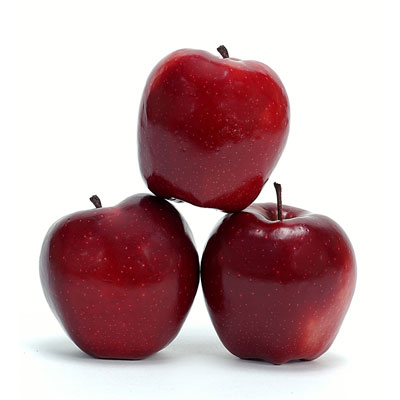
\includegraphics[width=4cm,height=4cm]{images/apples.jpg}
      \end{column}
      \begin{column}{5cm}
         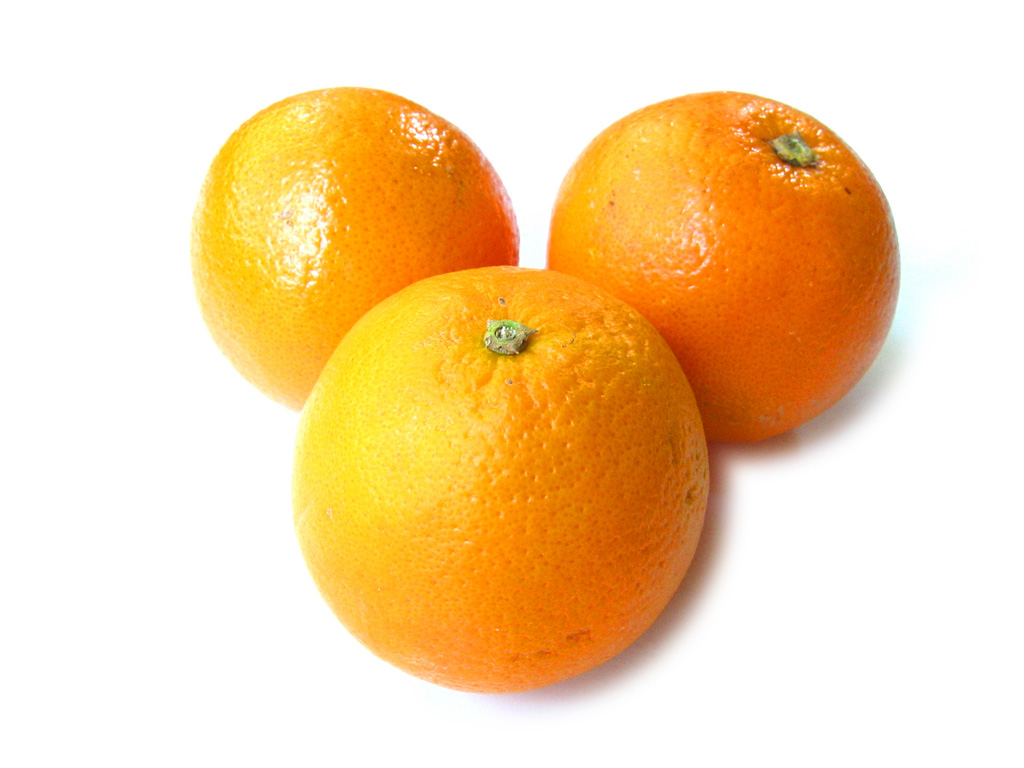
\includegraphics[width=4cm,height=3cm]{images/oranges.jpg}
      \end{column}
   \end{columns}
\end{frame}

\begin{frame}
   \frametitle{What is a Natural Number?}
   1858: Giuseppe Peano born\\
\end{frame}

\begin{frame}
\end{frame}
\end{comment}

\end{document}

